\chapter{Evaluation}
We evaluate our method based on the development data set from the ChAirGest
corpus~\cite{Ruffieux2013} with gestures captured from 10 users. There are
10 different gestures and 3 resting positions. There are 900 total gesture
occurrences (3 recording sessions for each user) in the development data set representing three forth of the entire corpus. The remaining one forth of the corpus are not released to
the public, and can be used for final evaluation on unseen data.

In this data set, on average, the hand is at 1.2m away
from the sensor, which means the depth error is around 5mm.

A frame-based accuracy score can be biased because a classifier that
favors longer gestures would have higher accuracy.

\textit{Precision} (P) corresponds to the number of correctly detected events
divided by the number of returned events and the \textit{Recall} metric
corresponds to the number of correctly detected events divided by the number of
events in the ground truth. \cite{Ruffieux2013}

\begin{align}
F1 = 2\times\frac{P \times R}{P + R}
\end{align}

\begin{table}[h]
\begin{center}
\begin{tabular}{|l|p{2cm}|p{1.7cm}|p{1.7cm}|}
\hline
 & Hand position from salience detection \& Xsens & Hand position
 from Kinect skeleton \& Xsens & Xsens Only \\
\hline
F1 Score & \textbf{0.907 (0.01)} & 0.870 (0.02) & 0.890 (0.02) \\
\hline
ATSR Score & \textbf{0.923 (0.02)} & 0.930 (0.03) & 0.920 (0.01) \\
\hline
Final Score & \textbf{0.912 (0.01)} & 0.881 (0.01) & 0.895 (0.01) \\
\hline
\end{tabular}
\caption{Comparison of the average 3-fold cross validation results for different
feature vectors. Values in parentheses are standard deviations.}
\label{tab:comp-feature}
\end{center}
\end{table}

If we only use motion features such as relative position, velocity and
acceleration, the result is poor because it cannot distinguish gestures with
the same path but different hand postures such as ``Wave Hello'' and ``Shake
Hand'', ``Circle Palm Rotation'' and ``Circle Palm Down''.

\begin{table}[h]
\begin{center}
\begin{tabular}{|l|p{2cm}|p{2cm}|p{1.7cm}|p{1.7cm}|}
\hline
          & motion & color & depth & both \\
\hline
F1 Score & 0.677 (0.04) & 0.703 (0.01) & 0.720 (0.02) & 0.723 (0.01) \\
\hline
ATSR Score & 0.893 (0.02) & 0.870 (0.01) & 0.880 (0.01) & 0.873 (0.01) \\
\hline
Final Score & 0.710 (0.03) & 0.732 (0.01) & 0.748 (0.01) & 0.749 (0.00) \\
\hline
\end{tabular}
\caption{Comparison of the average 3-fold cross validation results for
features from color and depth sensors. Values in parentheses are standard
deviations.}
\label{tab:comp-feature}
\end{center}
\end{table}

\begin{figure}[h]
\centering
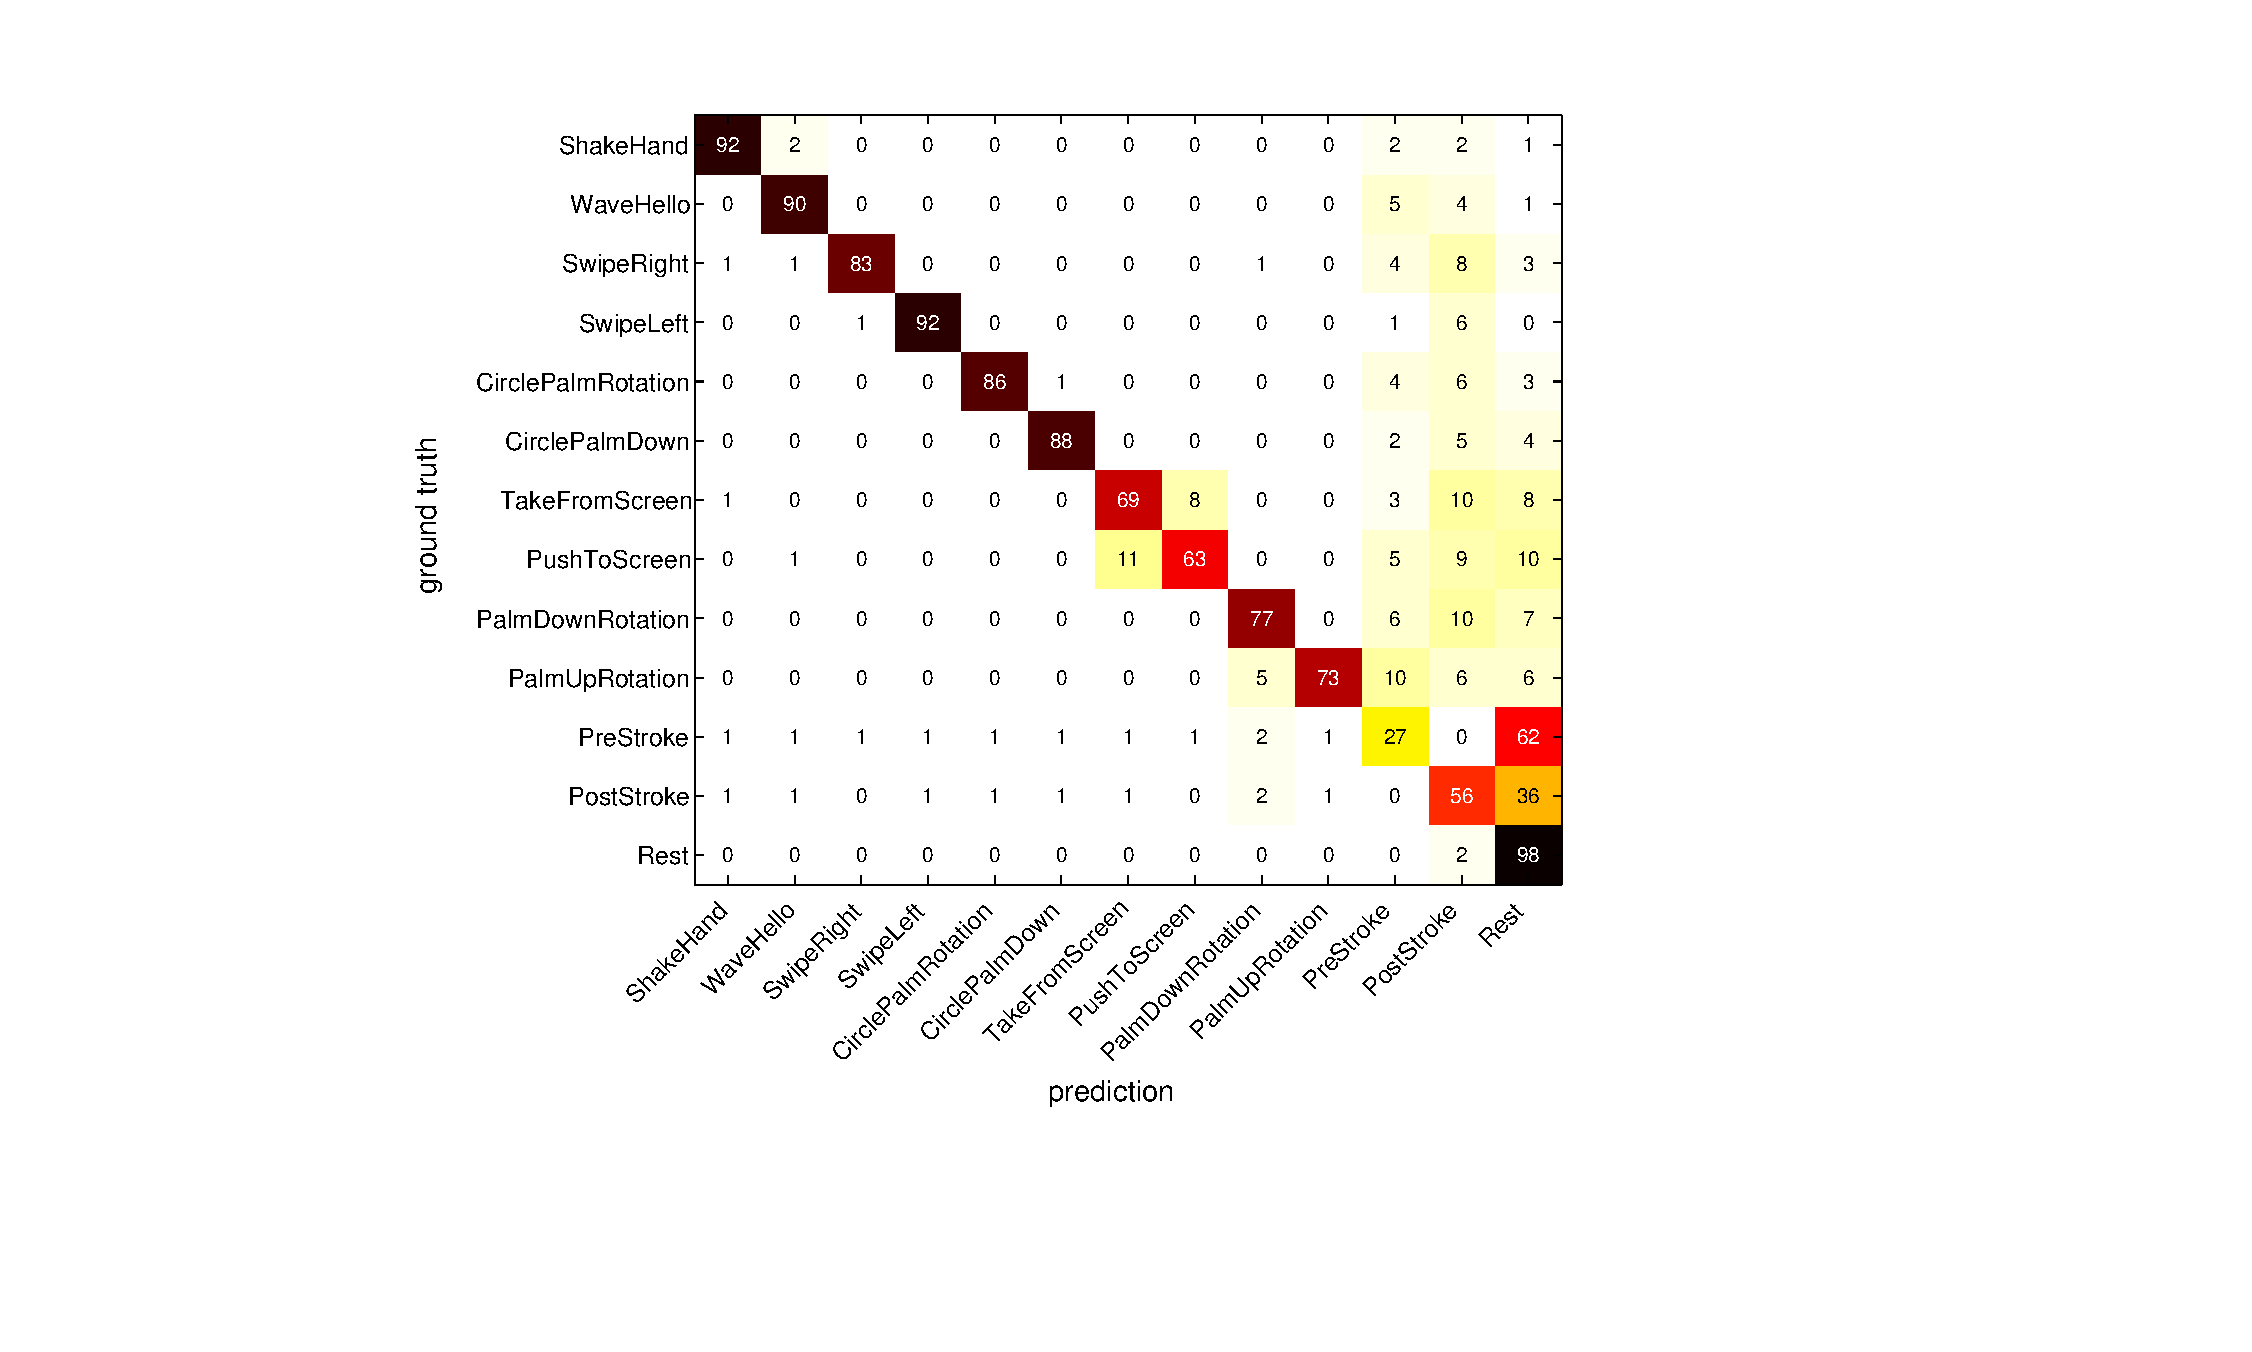
\includegraphics[trim={6cm 3.5cm 10cm 1.5cm}, clip,
width=0.5\columnwidth]{figures/confusion-matrix.eps} \caption{Per frame
classification confusion matrix based on result from 3-fold cross validation using both Kinect and Xsens features. The numbers are percentages. The darker the color the higher the percentage.}
\label{fig:confusion}
\end{figure}

\begin{figure}[h]
\centering
\includegraphics[trim={6cm 3.5cm 10cm 1.5cm}, clip,
width=0.6\columnwidth]{figures/confusion_motion.eps} \caption{Per frame
classification confusion matrix based on result from 3-fold cross validation
using motion features only (relative position, velociy, acceleration). The
numbers are percentages.
The darker the color the higher the percentage.}
\label{fig:confusion}
\end{figure}

\begin{figure}[tb]
\centering
\includegraphics[trim={6cm 3.5cm 10cm 1.5cm}, clip,
width=0.6\columnwidth]{figures/confusion_color_depth.png} \caption{Per frame
classification confusion matrix based on result from 3-fold cross validation using 
both color and depth images for hand. The numbers are percentages. The darker
the color the higher the percentage.}
\label{fig:confusion}
\end{figure}

``Take from Screen'' and ``Push to Screen'' have the lowest recognition
accuracy, especially when using the kienct data. We notice that when the users
extend their hands towards the screen, the hands are too close to the sensor
(below the too near range), and the depth sensor cannot get accurate readings.

